\documentclass[
  captions=tableheading,
  bibliography=totoc, 
  titepage=firstiscover,
]{scrartcl}

\usepackage{blindtext} %neuer input

\usepackage{longtable} % Tabellen über mehrere Seiten

\usepackage[utf8]{inputenc} %neuer input

\usepackage{scrhack}

\usepackage[aux]{rerunfilecheck} %Warnung falls nochmal kompiliert werden muss

\usepackage{fontspec} %Fonteinstellungen

\recalctypearea{}

\usepackage[main=ngerman]{babel} %deutsche Spracheinstellung

\usepackage{ragged2e} %neuer input

\usepackage{amsmath, nccmath}

\usepackage{amssymb} %viele mathe Symbole

\usepackage{mathtools} %Erweiterungen für amsmath


\DeclarePairedDelimiter{\abs}{\lvert}{\rvert}
\DeclarePairedDelimiter{\norm}{\lVert}{\rVert}

\DeclarePairedDelimiter{\bra}{\langle}{\rvert}
\DeclarePairedDelimiter{\ket}{\lvert}{\rangle}

\DeclarePairedDelimiterX{\braket}[2]{\langle}{\rangle}{
#1 \delimsize| #2
}

\NewDocumentCommand \dif {m}
{
\mathinner{\symup{d} #1}
}


\usepackage[
  math-style=ISO,
  bold-style=ISO,
  sans-style=italic,
  nabla=upright,
  partial=upright,
  warnings-off={
    mathtools-colon,
    mathtools-overbracket,
  },
]{unicode-math}

\setmathfont{Latin Modern Math}
\setmathfont{XITS Math}[range={scr, bfscr}]
\setmathfont{XITS Math}[range={cal, bfcal}, StylisticSet=1]


\usepackage[
  locale=DE,
  separate-uncertainty=true,
  per-mode=reciprocal,
  output-decimal-marker={,},
]{siunitx}

\usepackage[autostyle]{csquotes} %richtige Anführungszeichen

\usepackage{xfrac}

\usepackage{float}

\floatplacement{figure}{htbp}

\floatplacement{table}{htbp}

\usepackage[ %floats innerhalb einer section halten
  section,   %floats innerhalb er section halten
  below,     %unterhalb der Section aber auf der selben Seite ist ok
]{placeins}

\usepackage[
  labelfont=bf,
  font=small,
  width=0.9\textwidth,
]{caption}

\usepackage{subcaption} %subfigure, subtable, subref

\usepackage{graphicx}

\usepackage{grffile}

\usepackage{booktabs}

\usepackage{microtype} %Verbesserungen am Schriftbild

\usepackage[
backend=biber,
]{biblatex}

\addbibresource{../lit.bib}

\usepackage[ %Hyperlinks im Dokument
  german,
  unicode,
  pdfusetitle,
  pdfcreator={},
  pdfproducer={},
]{hyperref}

\usepackage{bookmark}

\usepackage[shortcuts]{extdash}

%\usepackage{warpcol}

\usepackage{tikz}

\newcommand*\circled[1]{\tikz[baseline=(char.base)]{
            \node[shape=circle,draw,inner sep=2pt] (char) {#1};}}

\begin{document}
    \title{V903 Doppler-Sonographie}
    \author{  
    Tobias Rücker\\
    \texorpdfstring{\href{mailto:tobias.ruecker@tu-dortmund.de}{tobias.ruecker@tu-dortmund.de}
    \and}{,} 
    Paul Störbrock\\
    \texorpdfstring{\href{mailto:paul.stoerbrock@tu-dortmund.de}{paul.stoerbrock@tu-dortmund.de}}{}
    }
    \date{Durchführung: 07.07.2020, Abgabe: 16.07.2020\vspace{-4ex}}
\maketitle
\center{\Large Versuchsgruppe: \textbf{23}}
    
\newpage
\tableofcontents
\newpage

\setcounter{page}{1}

\section{Ziel}

\section{Theorie}

    \flushleft{Die\;}\justifying Doppler-Sonographie nutzt den Doppler-Effekt aus um den Fluss innerhalb eines geschlossenen Systems bestimmen zu können. Der Doppler-Effekt 
    beschreibt die Streckung, bzw. Stauchung einer Wellenlänge im bewegten Bezugssystem. Bewegt sich die Quelle auf den Beobachter zu, wird die Wellenlänge gestaucht, also die
    Frequenz $\nu_0$ zu $\nu_{\text{gr}}$ vergrößert. Umgekehrt vergrößert sich die Wellenlänge sobald sich die Quelle von dem Beobachter wegbewegt, wodurch die Frequenz kleiner wird 
    $\nu_{\text{kl}}$. Daraus ergibt sich das folgende Verhältnis für die jeweils enstehende Frequenz: \cite{V903}
    \begin{align}
        \nu_{\text{gr,kl}} &= \frac{\nu_0}{1\mp \frac{v}{c}} \label{eq:1}
    \end{align}
    \flushleft{Hierbei\;}\justifying ist $v$ die Geschwindigkeit, mit welcher sich der Beobachter auf die Quelle zu, bzw. von der Quelle wegbewegt und $c$ die Schallgeschwindigkeit.
    Im Falle, dass sich die Quelle in Ruhelage befindet und sich der Beobachter auf die Quelle zu, bzw. von der Quelle wegbewegt, lässt sich ein ähnliches 
    Verhältnis beobachte. Bewegt sich die Quelle auf den Beobachter zu, wird die Frequenz $\nu_0$ zu $\nu_h$ angehoben. Ebenso wird die Frequenz $\nu_0$ bei einer sich vom Beobachter 
    wegbewegenden Quelle auf $\nu_n$ gesenkt. Das daraus entstehende Verhältnis lautet wie folgt: \cite{V903}
    \begin{align}
        \nu_{\text{h,n}} &= \nu_0 \left( 1\pm \frac{v}{c} \right) \label{eq:2}
    \end{align}
    \flushleft{Bei\;}\justifying der Doppler-Sonographie werden Ultraschallwellen an einem sich bewegenden Teilchen wie einem Blutkörperchen reflektiert. Die Bewegung des Blutkörperchens
    verursacht eine Frequenzverschiebung der Schallwelle, welche mit dem folgenden Aufbau zu messen ist.

\begin{figure}[H]
    \centering
    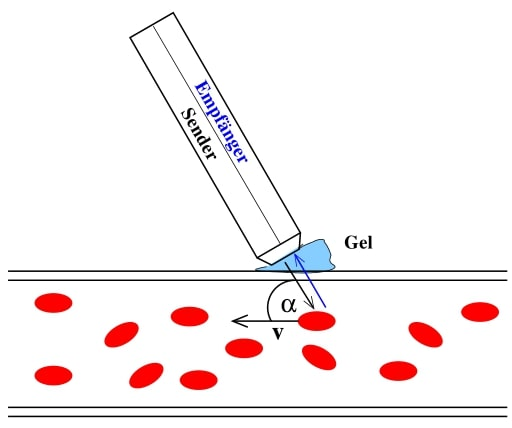
\includegraphics[width=0.5\linewidth]{images/Schema.jpg}
    \caption{In dieser schematischen Darstellung der Doppler-Sonographie \cite{V903} ist eine Sonde dagestellt. Diese beinhaltet einen Sender und einen Empfänger von Ultraschallwellen.
    Die Wellen fallen in einen Fluss von Teilchen (hier der Doppler-Flüssigkeit) ein und werden dort reflektiert. Der Winkel zwischen Wellennormalen und Geschwindigkeitsvektor des Teilchen ist $\alpha$
    oder $\beta$. Es wird bei den Winkeln zwischen einfallender und ausfallender Welle unterschieden, die in diesem Aufbau jedoch einen identischen Winkel besitzten. Das Gel sorgt dafür,
    das die Schallwellen nicht von der Luft absorbiert werden.}
    \label{fig:1}
\end{figure}

    \flushleft{In\;}\justifying diesem Aufbau sind die Winkel $\alpha$ und $\beta$ zwischen Geschwindigkeitsvektor $v$ und den Wellennormalen der einfallenden und reflektierten Welle identisch. Die 
    entstehende Frequenzverschiebung $\Delta\nu$ lautet demnach wie folgt:
    \begin{align}
        \Delta\nu &= 2\cdot \nu_0 \frac{v}{c} \cos(\alpha) \label{eq:3}
    \end{align} 
    \flushleft{Die\;}\justifying Ultraschallwellen werden mithilfe des piezo-elektrischen Effekts gewonnen. Der piezo-elektrische Effekt beschreibt die Eigenschaft eines Piezokristalls,
    der in ein elektrisches Wechselfeld gehalten wird. Zeigt eine Polarachse des Kristalls in Richtung des E-Felds beginnt der Kristall zu schwingen. Diese Schwingung regen den Kristall an
    Ultraschallwellen abzustrahlen.
    Neben der Erzeugung von Ultraschallwellen kann ein Piezokristall auch als Empfänger verwendet werden, da Ultraschallwellen den Kristall ebenfalls zum schwingen bringen.\\
    Neben der Sonde wird noch ein Doppler-Prisma verwendet. Eine schemarische Darstellung ist in der folgende Abbildung zu finden:

\begin{figure}[H]
    \centering
    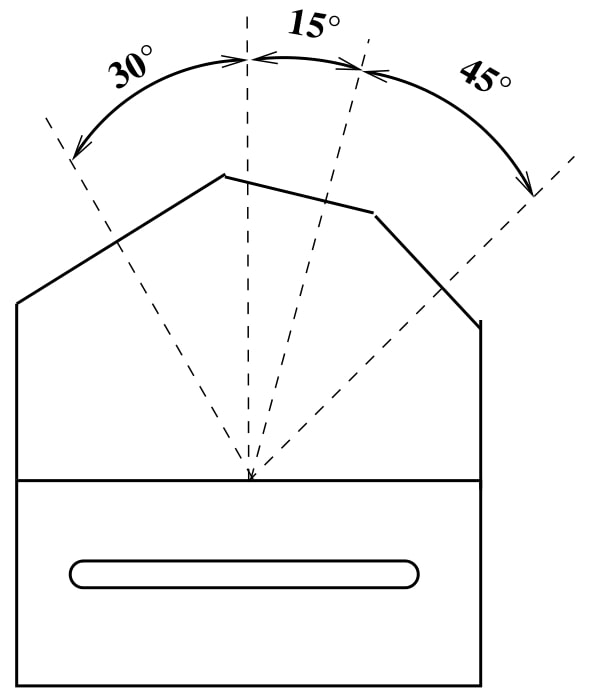
\includegraphics[width=0.35\linewidth]{images/Winkel.jpg}
    \caption{Diese Abbildung stellt das Doppler-Prisma dar \cite{V903}. Es erlaubt der Sonde drei Aufsetzmöglichkeiten, die jeweils einen festen Winkel zum darunterliegenden Rohr besitzen. Das
    Prisma ist so konstruiert, dass die Strecken zwischen Sonde und Rohr gleich bleibt. Die hier abgebildeten Winkel sind \SI{15}{\degree}, \SI{30}{\degree} und \SI{45}{\degree}.}
    \label{fig:2}
\end{figure}

    \flushleft{Da\;}\justifying mit dem Doppler-Prisma ein weiterer Brechungswinkel eingeführt wird und die Sonde an drei Winkeln fixiert wird, ergibt sich aud dem Brechungsgesetz
    für den Winkel $\alpha$: \cite{V903}
    \begin{align}
        \alpha &= \text{\SI{90}{\degree}} - \arcsin\left( \sin(\theta) \frac{c_L}{c_P} \right) \label{eq:4}
    \end{align}
    \flushleft{Hier\;}\justifying beschreibt der Winkel $\theta$ einen der drei fixierten Winkel \SI{15}{\degree}, \SI{30}{\degree}, oder \SI{45}{\degree}. $c_L$ ist die Schallgeschwindigkeit
    in der Doppler-Flüssigkeit und $c_P$ ist die Schallgeschwindigkeit des Prismenmaterials.

\newpage
\section{Vesuchsaufbau und Durchführung}

    \flushleft{Für\;}\justifying den Versuch wird folgender Versuchsaufbau verwendet:

\begin{figure}[H]
    \centering
    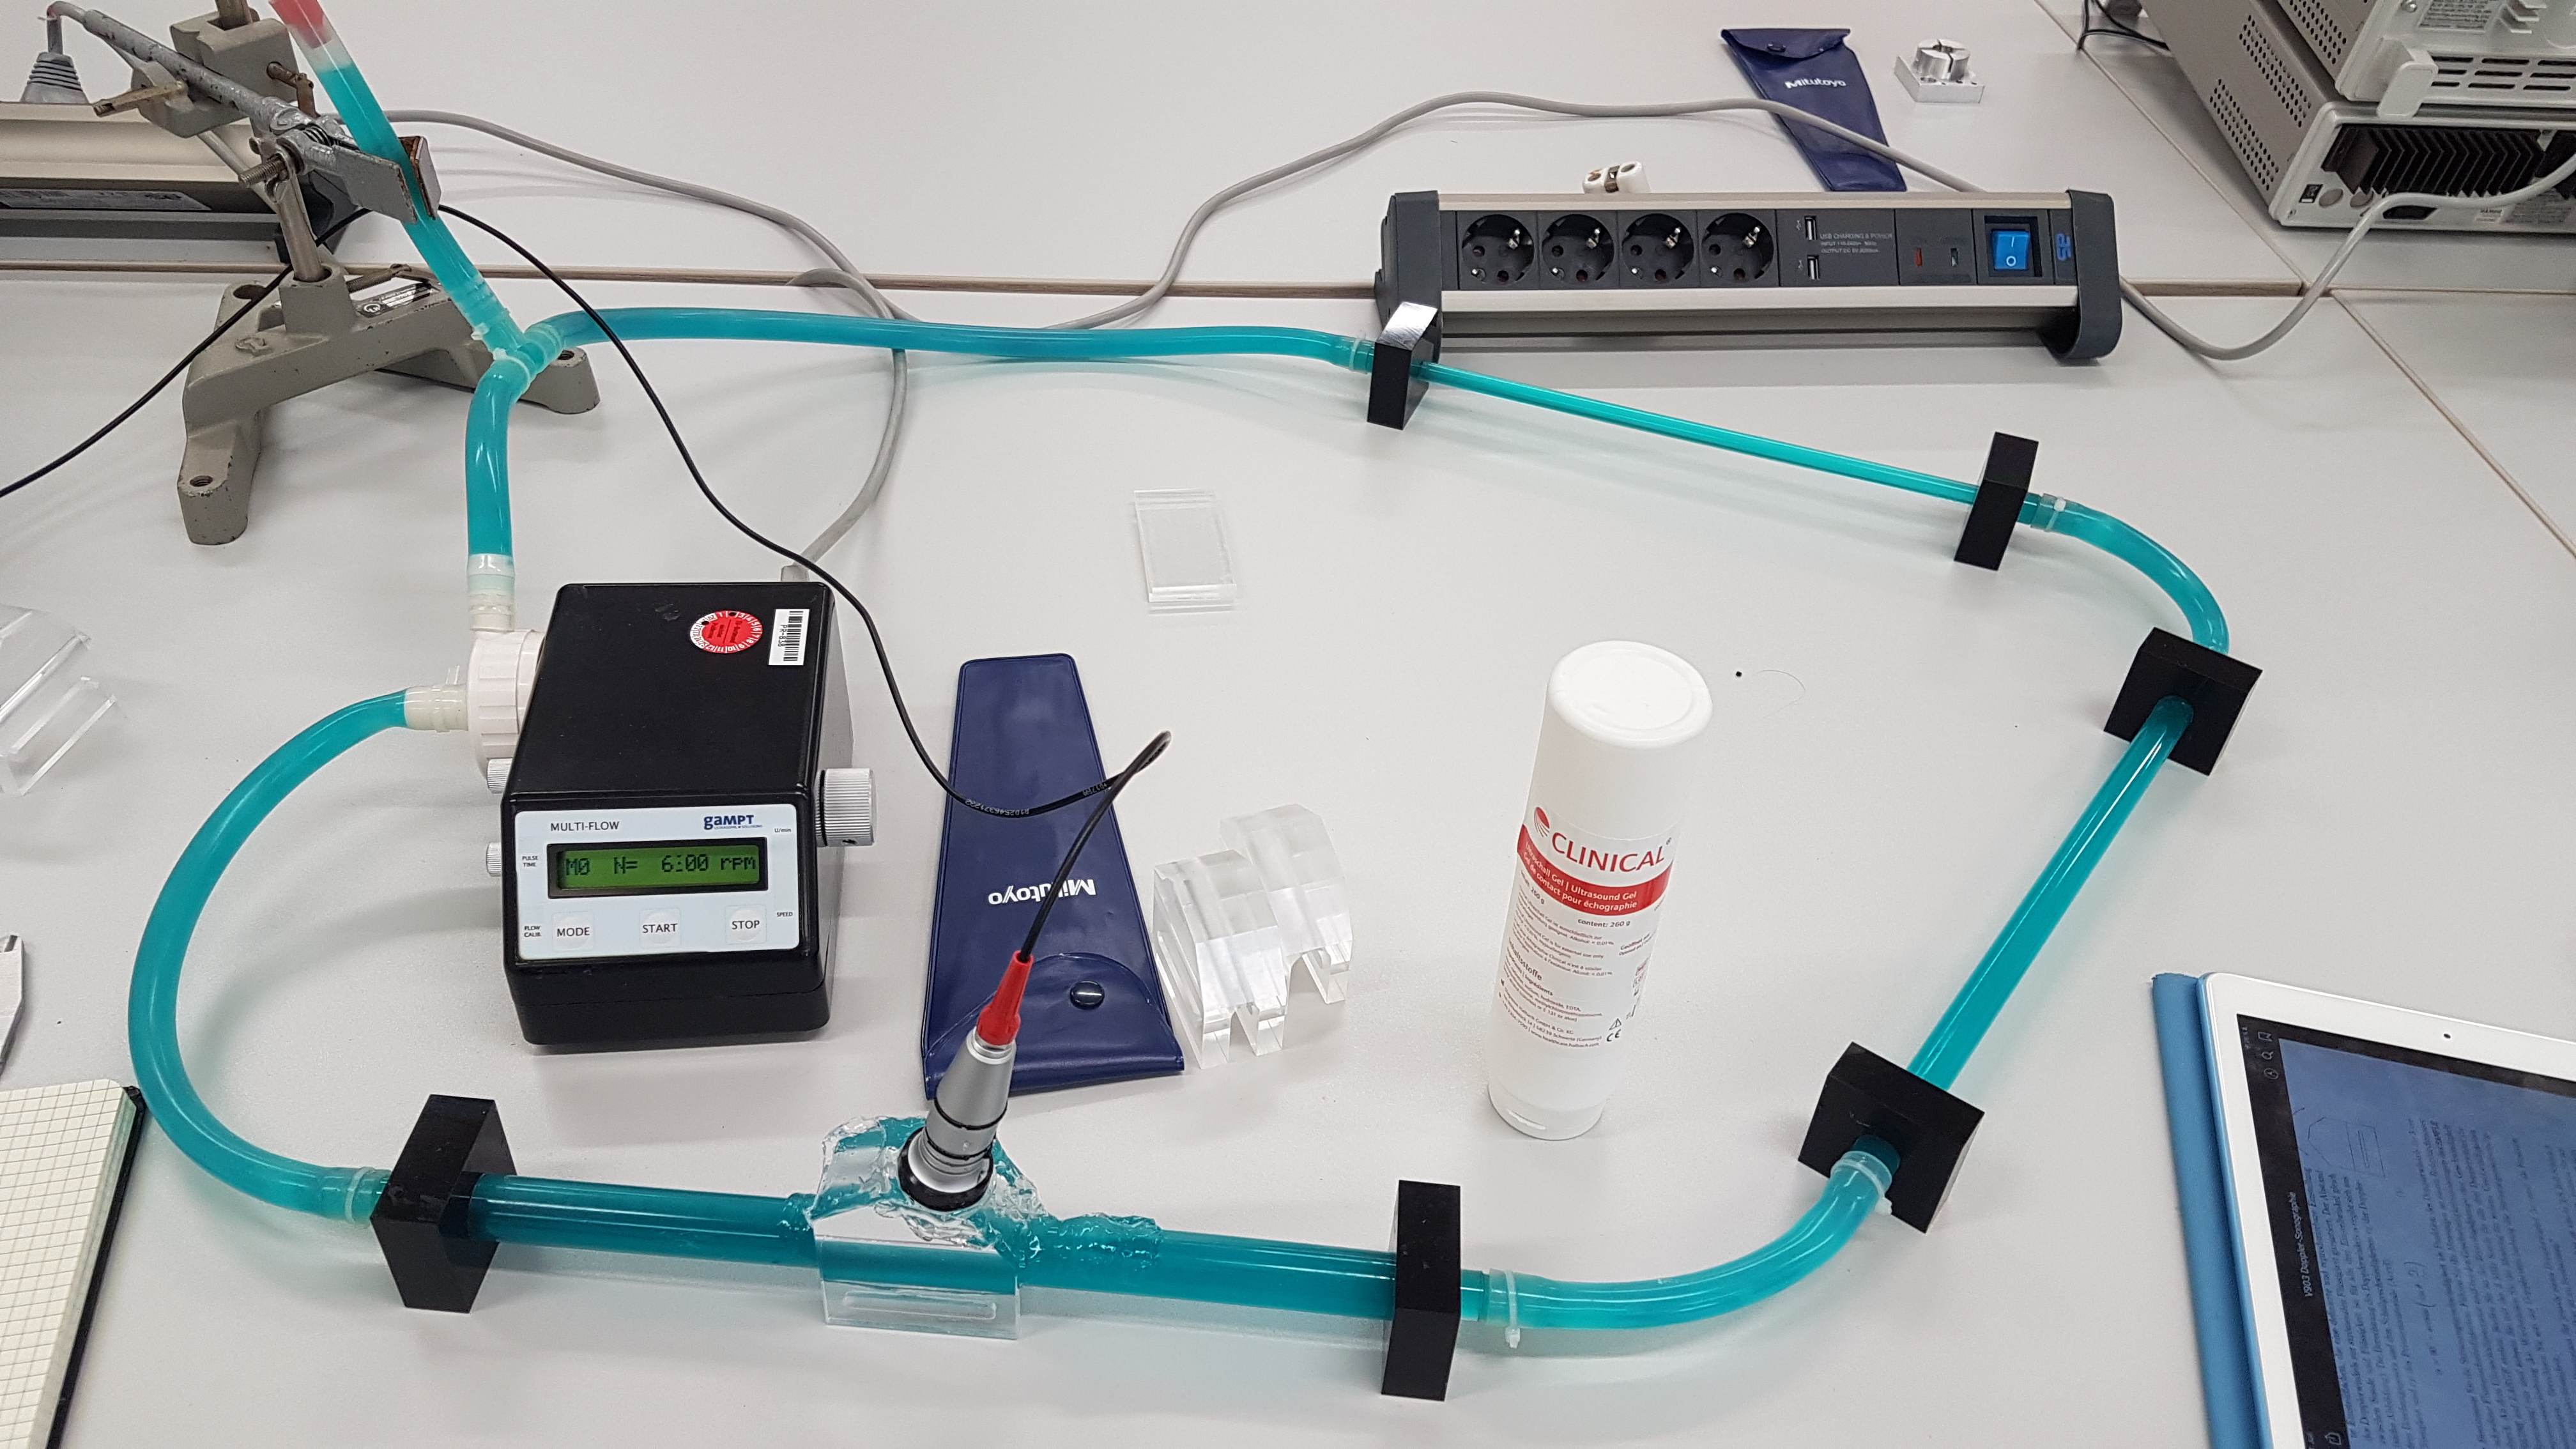
\includegraphics[width=0.75\linewidth]{images/Schlauch.jpg}
    \caption{In dieser Abbildung ist der Aufbau des Versuches zu erkennen. Der Versuch besteht aus einem Schlauch, der in vier Teile zerlegt werden kann. Ganz links befindet sich die 
    Pumpe, welche die Doppler-Flüssigkeit mit verschiedenen Stärken durch den Schlauch pumpen kann. Die Stärke kann dem Display der Pumpe entnommen werden. Unten mittig befindet sich
    das große Rohr mit einem Außendurchmesser von \SI{2.015}{\centi\meter}, welcher mit der sich über dem Rohr befindlichen Schieblehre gemessen wurde. Auf das Rohr selbst ist das 
    Doppler-Prisma aufgesetzt, worauf sich die Sonde befindet. Sowie zwischen Sonde und Prisma, als auch zwischen Prisma und Rohr ist Gel aufgetragen. Wird der Schlauch gegen den 
    Uhrzeigersinn verfolgt sind die anderen beiden Rohre mit abnehmender Dicke zu finden. Das für diesen Versuch relevante Rohr ist jedoch das dicke Rohr mit dem aufgesetzten Prisma.}
    \label{fig:3}
\end{figure}
\begin{figure}[H]
    \centering
    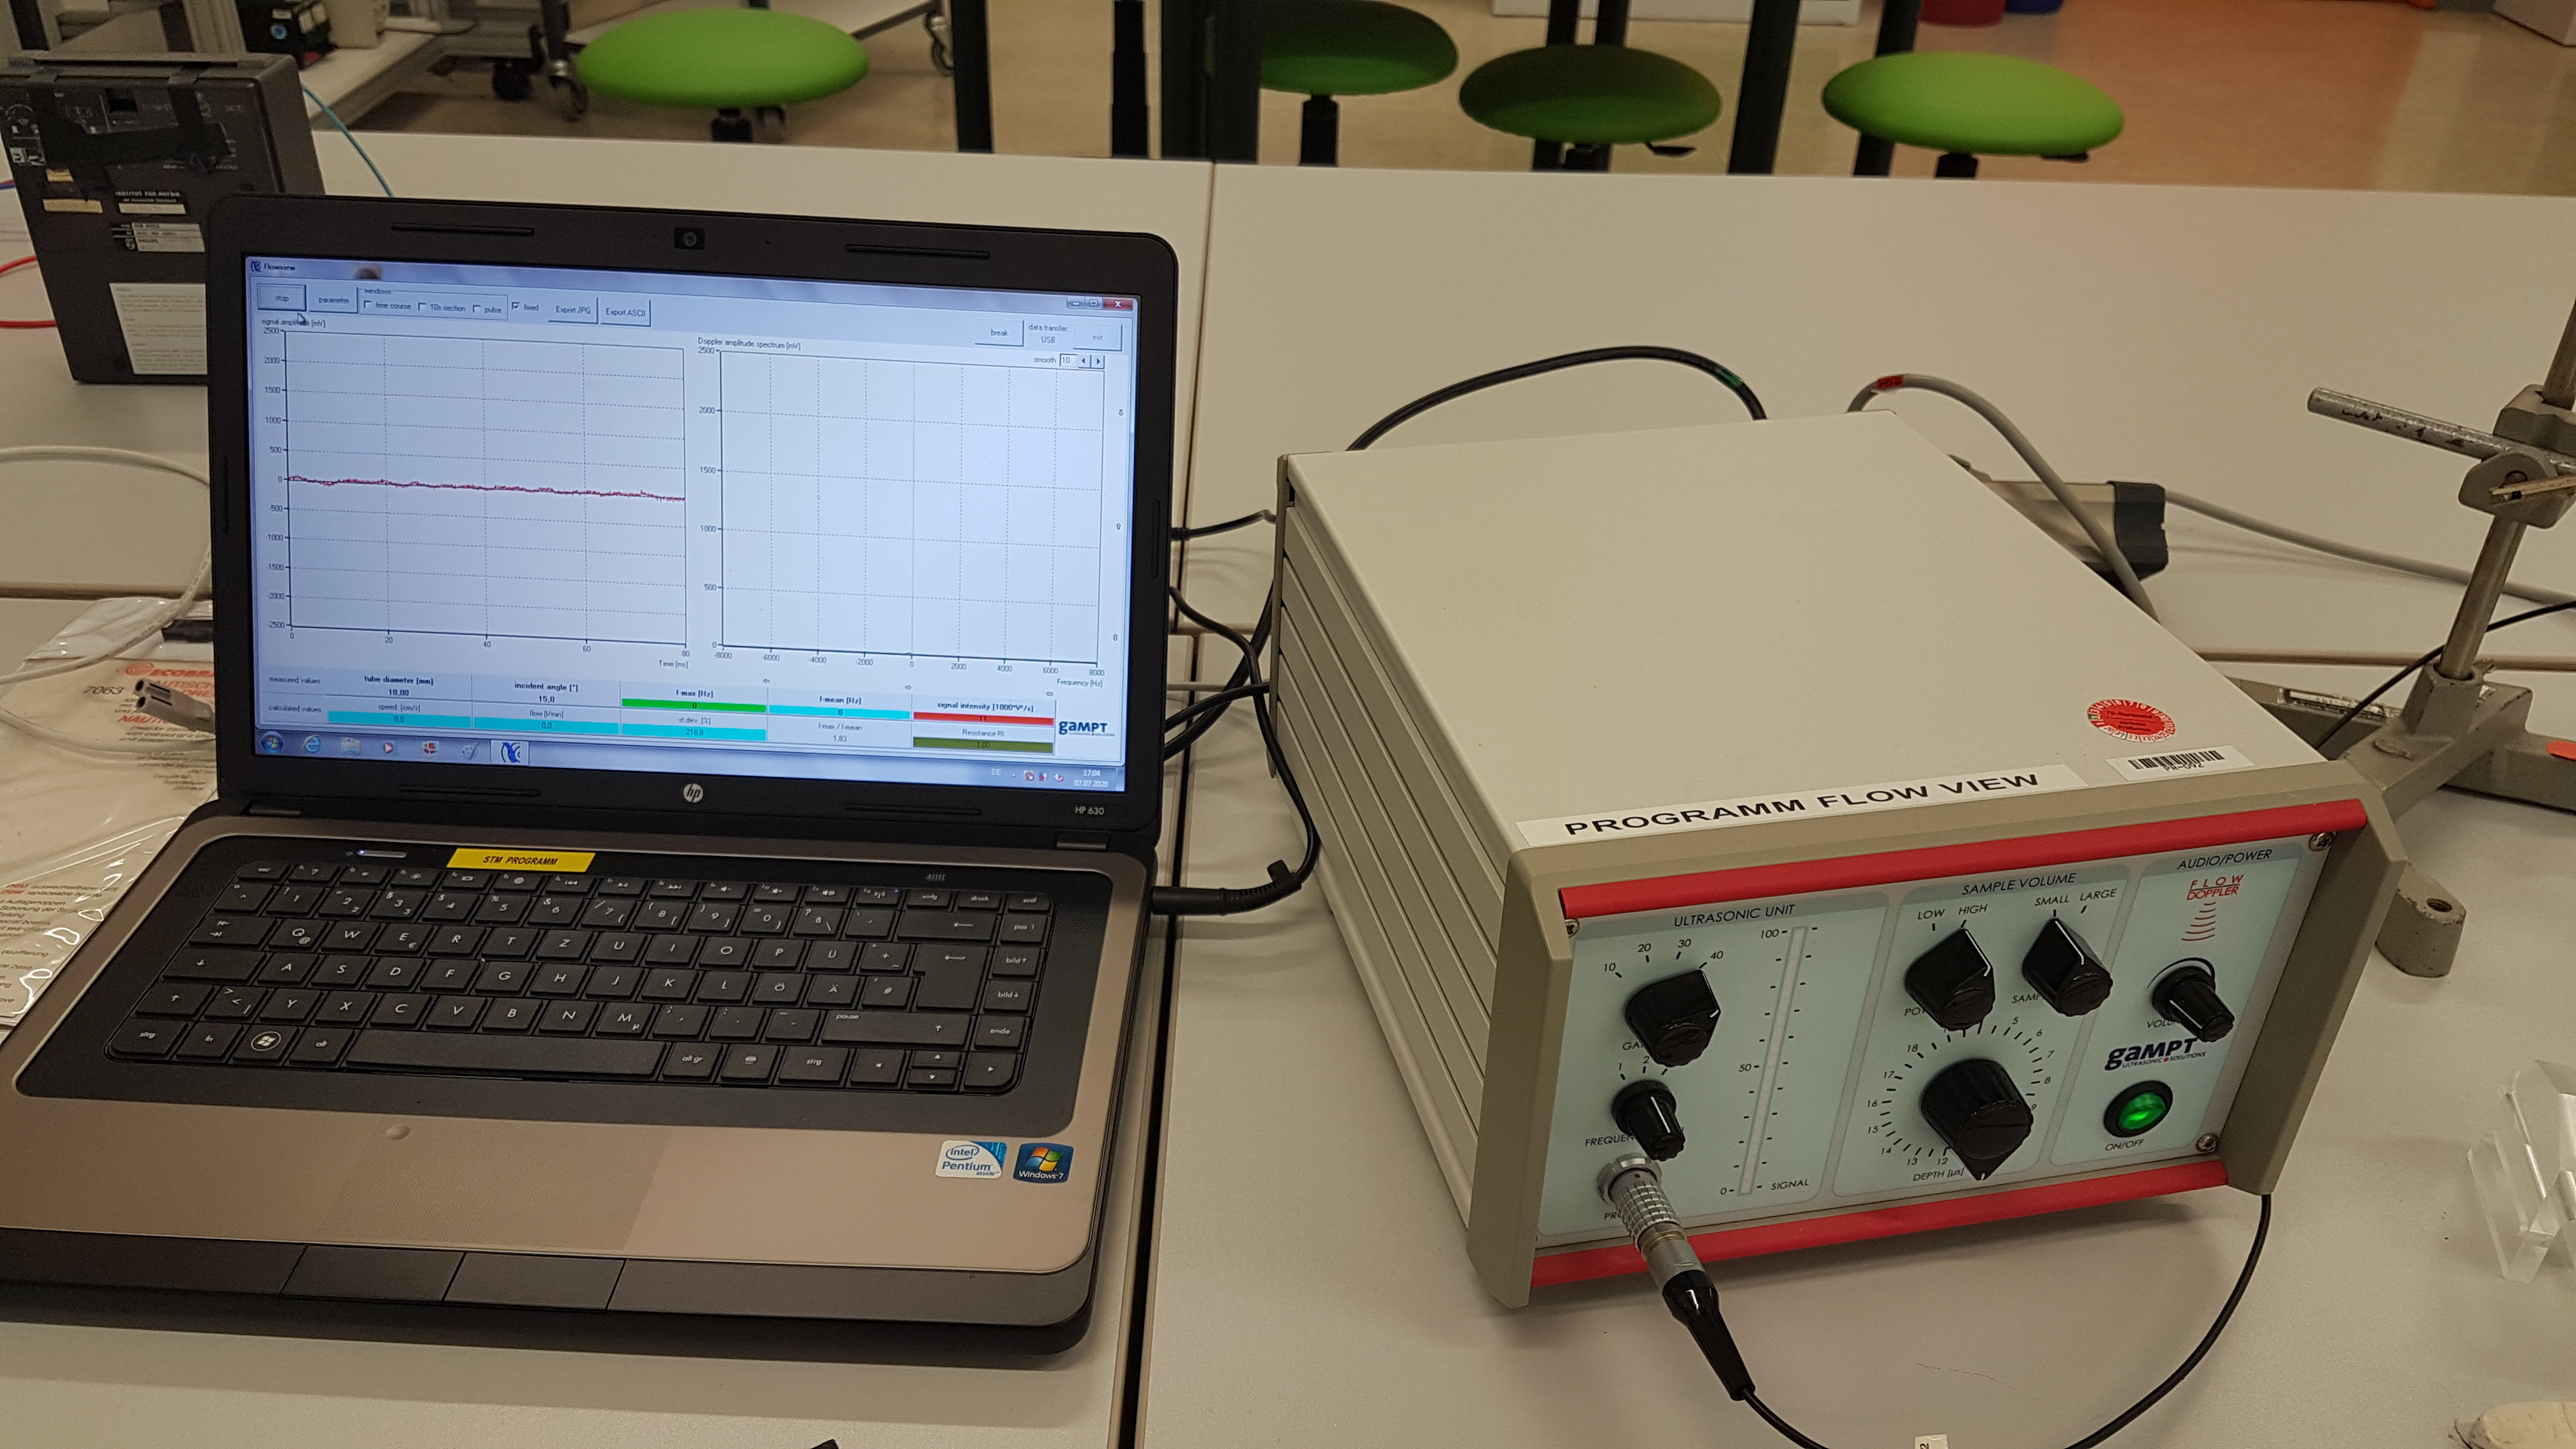
\includegraphics[width=0.75\linewidth]{images/Messaperatur.jpg}
    \caption{Hier ist die Messaperatur der Sonde abgebildet. Auf dem Laptop ist das UI des Programms FlowView zu erkennen, welches die Daten des rechts befindlichen Ultraschallgenerator 
    ausließt. Am Ultraschallgenerator kann zwischen den Einstellungen \textit{Small} und \textit{Large} unterschieden werden, welche für das Strömungsprofil und die Strömungsstärke relevant sind.
    Außerdem kann die Messtiefe unter der Einstellungen \textit{Small} variiert werden, was die Bestimmung des Strömungsprofils ermöglicht.}
    \label{fig:4}
\end{figure}

    \flushleft{Zu\;}\justifying Beginn wird der Ultraschallgenerator aus Abbildung \ref{fig:4} auf \textit{Large} gestellt um die Strömungsgeschwindigkeit bestimmen zu können. Anschließend wird zwischen
    dem Doppler-Prisma und dem Rohr Gel aufgetragen. Das gleiche wird für die Sonde an den drei Aufsetzpunkten wiederholt. Dann werden für die drei Winkel \SI{15}{\degree}, 
    \SI{30}{\degree} und \SI{45}{\degree} die Frequenzverschiebung $\Delta\nu$ dem Laptop entnommen. Dafür werden an der Pumpe nacheinander fünf Stärken eingestellt, für die jeweils ein Messwert 
    für die Frequenzverschiebung am Laptop abgelesen wird. Dies wird für jeden der drei Winkel wiederholt. Die fünf Stärken der Pumpe bleiben für alle drei Winkel gleich.\\
    Für das Strömungsprofil wird der Ultraschallgenerator auf \textit{Small} eingestellt. Es wird in dem Messintervall \SI{13.5}{\micro\second} bis \SI{19.5}{\micro\second} in \SI{0.5}{\micro\second} Schritten die 
    Frequenzverschiebung $\Delta\nu$ und die dazugehörige Signalstärke gemessen. 

\newpage
\section{Auswertung}

    \flushleft{Alle\;}\justifying folgenden Graphen werden mit der Python Bibliothek matplotlib \cite{matplotlib} und dem Befehl polyfit aus der numpy Bibliothek \cite{numpy} erstellt. 
    Alle Fehler werden mithilfe der python Bibliothek uncertainties \cite{uncertainties} berechnet.\\
    \flushleft{Um\;}\justifying auf die Strömungsgeschwindigkeit der Doppler-Flüssigkeit zu schließen wird die Formel der Frequenzverschiebung $\Delta\nu$ \eqref{eq:3} zur Geschwindigkeit
    $v$ umgestellt, wodurch sich für die Geschwindigkeit folgendes Verhältnis ergibt:
    \begin{align}
        v &= \frac{1}{2} \frac{\Delta\nu \cdot c_L}{\nu_0\cdot \cos(\alpha)} \label{eq:5}
    \end{align}

\subsection{Strömungsgeschwindigkeit für 15°}

    \flushleft{Aus\;}\justifying Formel \eqref{eq:5} lassen sich die Strömungsgeschwindigkeiten für die einzelnen Geschwindigkeiten der Pumpe bestimmen. Mit den Werten aus 
    Tabelle \ref{tab:1} für die Frequenzverschiebung $\Delta\nu$ und den daraus mit Formel \eqref{eq:5} berechneten Geschwindigkeiten lässt sich folgender Graph erstellen. Hier
    wird das Verhältnis $\sfrac{\Delta\nu}{\cos(\alpha)}$ gegen die jeweilige Strömungsgeschwindigkeit $v$ graphisch dargestellt, wobei der Dopplerwinkel $\alpha$ mit Formel 
    \eqref{eq:4} unter Verwendung des Winkels $\theta=15°$ bestimmt wird. Als Schallgeschwindigkeit wird hier die Schallgeschwindigkeit innerhalb der Doppler-Flüssigkeit
    $c_L=\text{\SI{1800}{\meter\per\second}}$ verwendet. 

\begin{figure}[H]
    \centering
    \includegraphics[width=0.75\linewidth]{build/plot15.pdf}
    \caption{}
    \label{fig:5}
\end{figure}

    \flushleft{Die\;}\justifying für diesen Graphen relevanten Parameter der Steigung $m$ und des Schnittpunkts mit der y-Achse $b$ lauten wie folgt:
    \begin{align}
        m_{15°} &= \text{\input{m15.tex}} \label{eq:6}\\
        b_{15°} &= \text{\input{b15.tex}} \label{eq:7}
    \end{align}



\begin{figure}[H]
    \centering
    \includegraphics[width=0.75\linewidth]{build/plot30.pdf}
    \caption{}
    \label{fig:6}
\end{figure}



\begin{figure}[H]
    \centering
    \includegraphics[width=0.75\linewidth]{build/plot45.pdf}
    \caption{}
    \label{fig:7}
\end{figure}



\begin{figure}[H]
    \centering
    \includegraphics[width=0.75\linewidth]{build/plotdepth.pdf}
    \caption{}
    \label{fig:8}
\end{figure}

\section{Diskussion}

\newpage
\printbibliography

\newpage
\section*{Appendix}
\addcontentsline{toc}{section}{Appendix}

\begin{table}[H]
    \centering
    \caption{Placeholder}
    \input{15.tex}
    \label{tab:1}
\end{table}

\begin{table}[H]
    \centering
    \caption{Placeholder}
    \input{30.tex}
    \label{tab:2}
\end{table}

\begin{table}[H]
    \centering
    \caption{Placeholder}
    \input{45.tex}
    \label{tab:3}
\end{table}

\begin{table}[H]
    \centering
    \caption{Placeholder}
    \input{data.tex}
    \label{tab:4}
\end{table}


\end{document}